\documentclass[discrete.tex]{subfiles}

\begin{document}
  \section{Теорема Кенига}

  \begin{definition}
      Вершинное покрытие графа - множество вершин, такое, что любое ребро графа
      имеет хотя бы одну конечную вершину из этого множества.
  \end{definition}

  \begin{definition}
      Вершинное покрытие называется наименьшим, если никакое другое вершинное покрытие не
      имеет меньшего числа вершин.
  \end{definition}

  \begin{theorem} [Кёнига]
      В любом двудольном графе число ребер в макс. паросочетании равно числу вершин в
      наименьшем вершинном покрытии
  \end{theorem}

  \begin{figure}[H]
          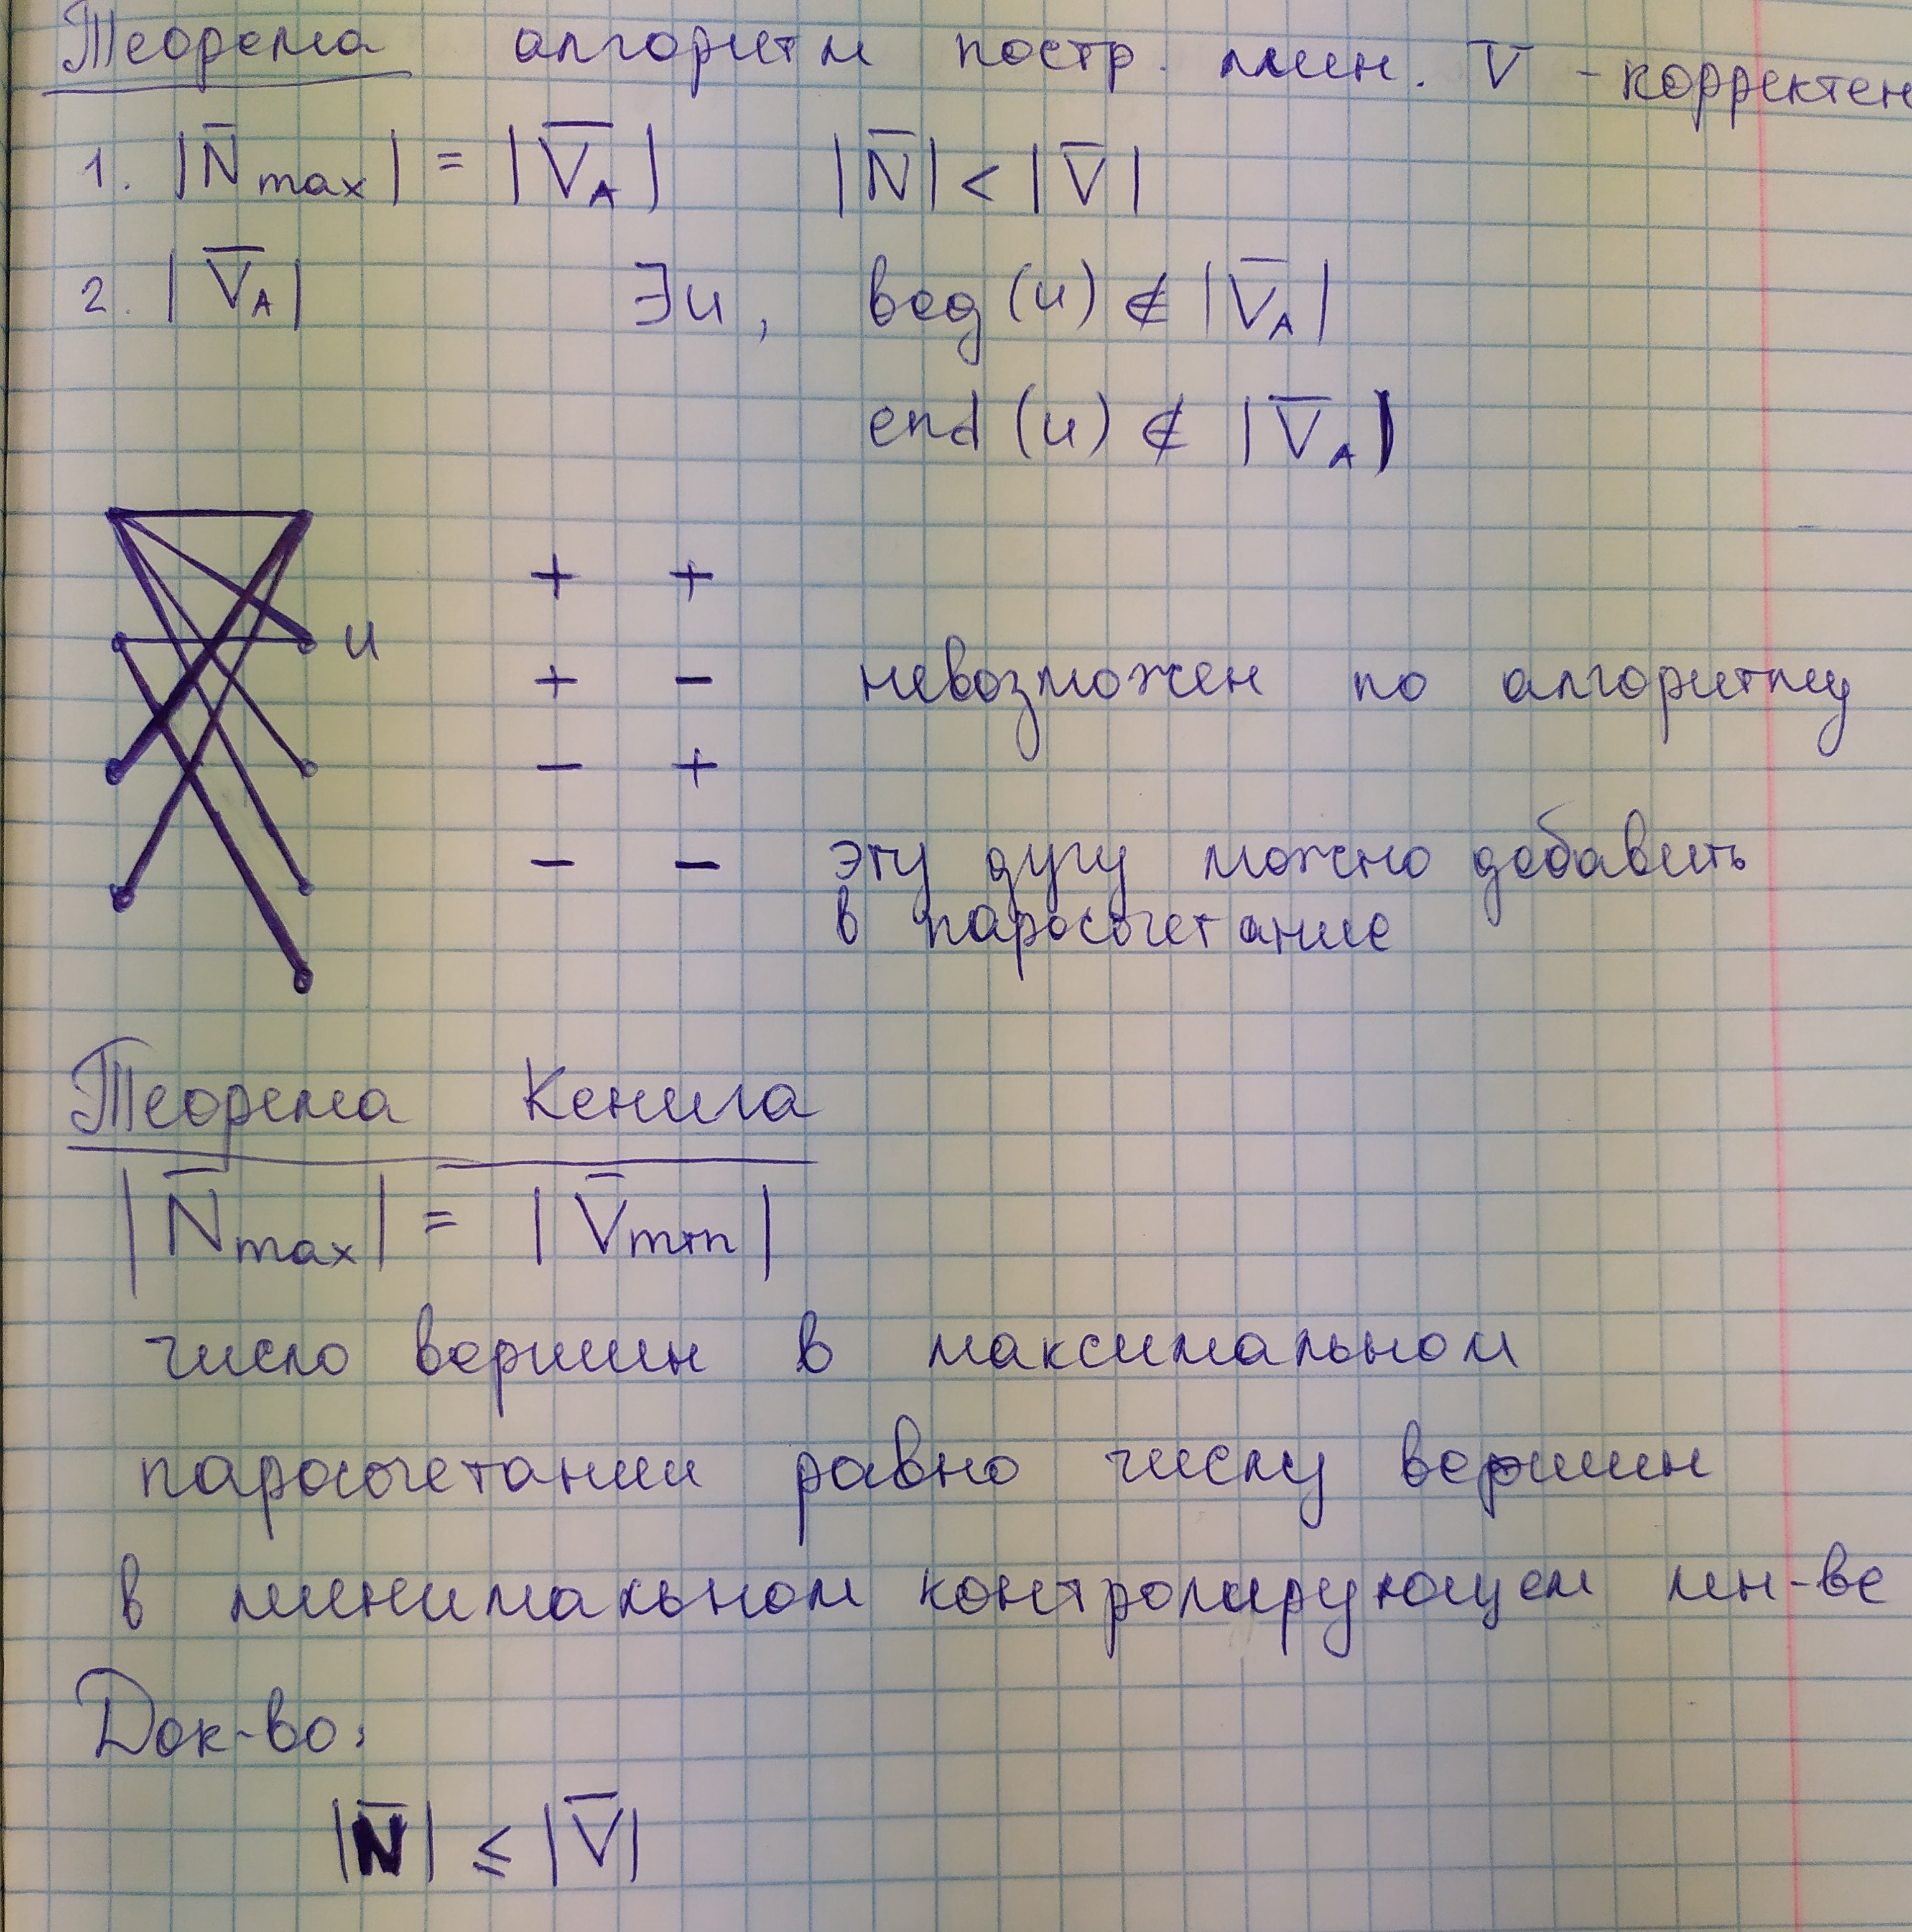
\includegraphics[width=10cm]{pics/50_1}
          \centering
  \end{figure}

  \begin{figure}[H]
          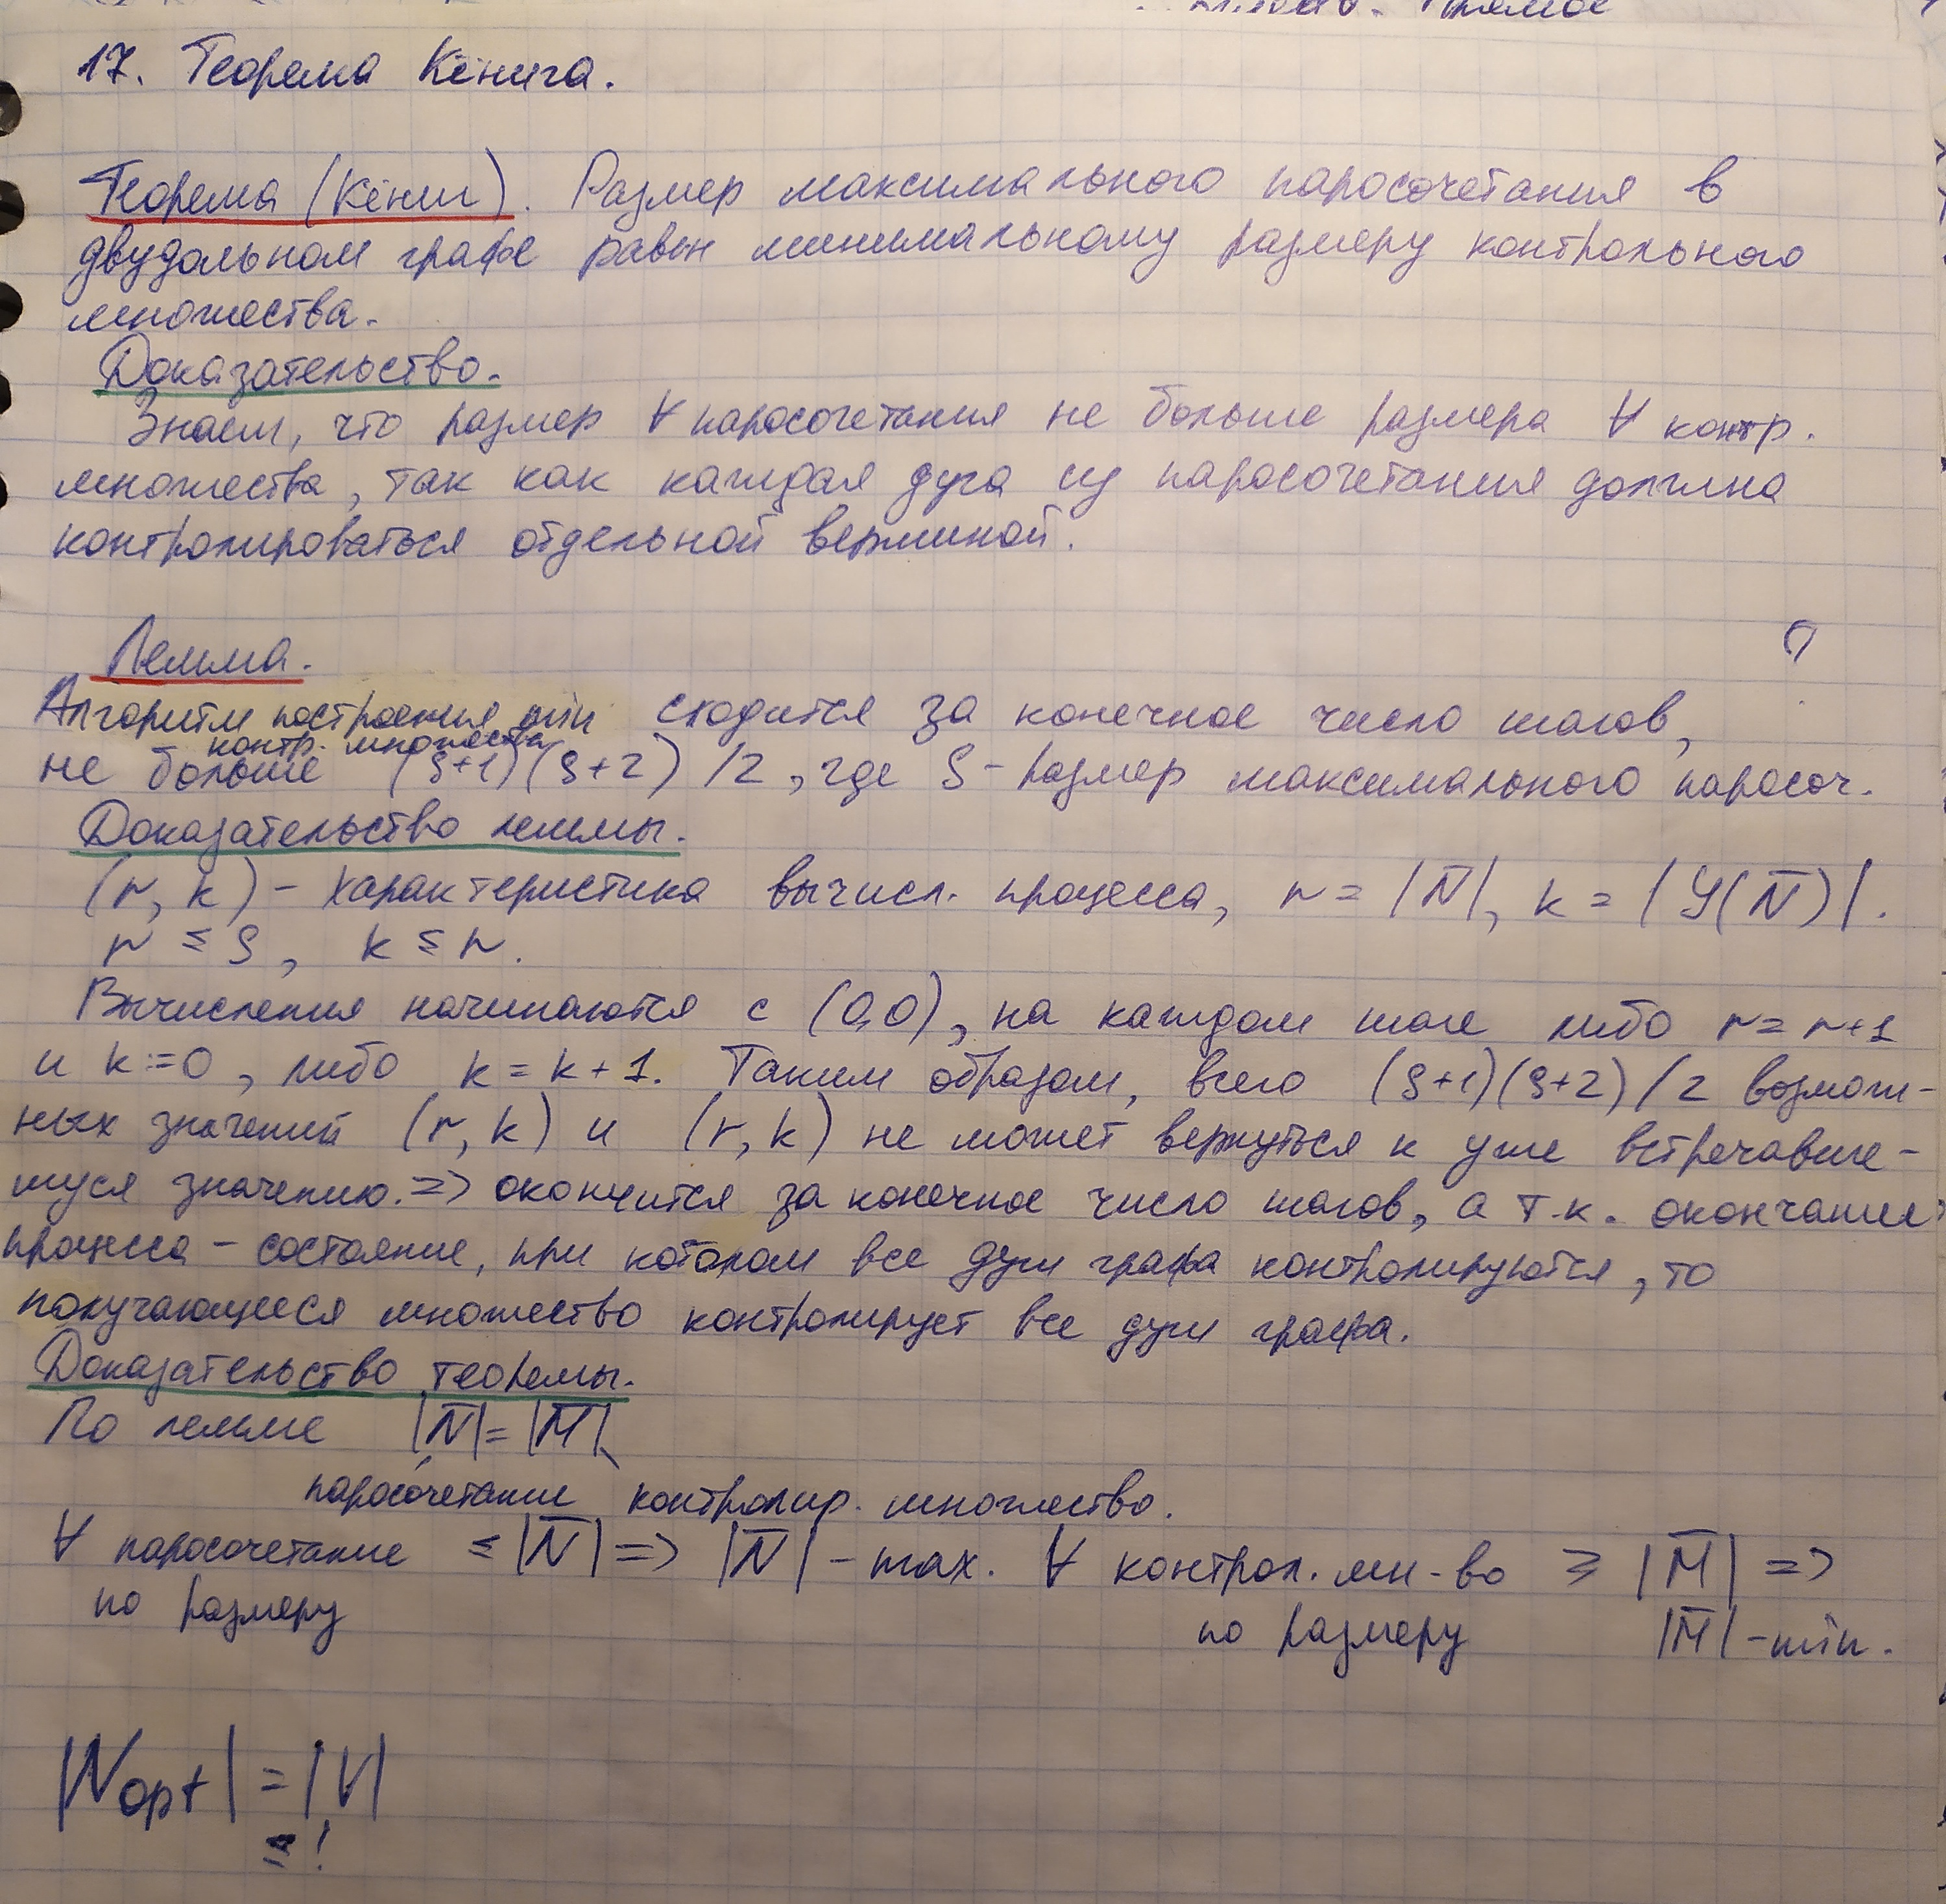
\includegraphics[width=10cm]{pics/50_2}
          \centering
  \end{figure}
\end{document}
